\documentclass[10pt]{article}

\usepackage{graphics,color}
% Note that png and jpg extensions are used for graphics
\DeclareGraphicsExtensions{.png,.jpg}


% Construct the basic page sizes
\oddsidemargin  0.0in
\evensidemargin 0.0in
\textwidth      6.5in
\headheight     0.25in
\topmargin      0.0in
\textheight=8.5in


\begin{document}

\title{Program Flow for a Propagation Enabled Command}
\author{Darrel J. Conway\\\textit{Thinking Systems, Inc.}\\
Steven P. Hughes\\\textit{Goddard Space Flight Center}}
\date{\today}
\maketitle

\begin{abstract}
This document described the interactions between the components used in GMAT to propagate objects.
\end{abstract}

\section{Introduction}

GMAT provides a collection of components that are tailored to advancing objects in GMAT's model over
time.  Users instruct GMAT about the types of objects that are expected to evolve, and the elements
of those objects that are needed by the model, using Mission Control Sequence commands that are
enabled for propagation.  The current design plan for GMAT identifies three propagation-enabled
commands: ``Propagate'', ``RunEstimator'', and ``RunSimulator''.  The discussion that follows will
examine the Propagate command in detail, and then discuss the other commands in the context of
propagation.

\section{Propagation Overview}

The commands governing propagation in GMAT all pass through five stages in the course of modeling a
mission.  These stages, shown in Figure~\ref{fig:PropLifetime}, start from the creation of the
command and run through its initialization, setup and execution, and completion and finalization.
The following paragraphs give an overview of each of these stages.

\begin{figure}[htb]
\begin{center}
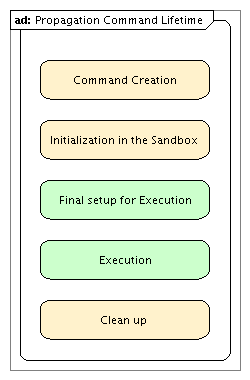
\includegraphics[125,190]{Images/PropagationCommandLifetime.png}
\caption{Stages in the Lifetime of a Propagation Enabled Command}
\label{fig:PropLifetime}
\end{center}
\end{figure}

\paragraph{Command Creation}

Propagation enabled commands are created following the same pattern as all other commands in GMAT.
A user creates the command, either through a line if text in a mission script file or function file
or from GMAT's graphical user interface using the panel for the command.  When the script is parsed
or the panel closed, GMAT creates an object based on that action, and passes that object the
detailed information necessary to configure the command.  This information is stored in string form
at this stage.  It identifies the interconnections that are needed to execute the command during a
mission run.  The command validates all of the information that can be checked locally at this
point.

\paragraph{Initialization}

The first step GMAT performs when running a mission is the initialization step in the Sandbox used
for the run.  During this phase of the run, all of the objects configured for the mission are cloned
into the Sandbox, and the mission control sequence is assigned to the Sandbox.  The objects are
initialized, and then each command in the control sequence is initialized.  During initialization,
all of the interconnections between components are set, and as much preparation as possible is made
to run the mission.  For propagation enabled commands, initialization includes cloning of the
configured propagators used in the command so that a local instance is available for propagation.
The parameters needed to execute the desired propagation are set, and the data needed for
propagation collected and validated.  The actual propagation state vector cannot be constructed at
this point because commands in the mission control sequence prior to the propagation enabled command
may affect that state vector.

\paragraph{Final Setup}

After initialization, the Sandbox starts running the Mission Control Sequence by executing the
commands sequentially.  For propagation enabled commands, the first action taken when execution is
requested is a final setup of the objects used for propagation.  This setup checks for changes to
the objects that affect the propagation state (for example, a transient force like a thruster firing
may have become active), builds the propagation state vector, establishes a mapping between the ODE
model and that state vector if the propagator needs it, and populates the state vector with the
initial data that is to be propagated.

\paragraph{Execution}

Once the final setup is complete, the command is ready to begin propagation.  Propagation is
performed a step at a time.  The propagator is asked for an integration step.  The step is taken and
the resulting state vector returned.  The command checks the result to see if a stopping point has
been reached.  If not, the objects are updated with the propagated information.  If a stopping point
was encountered in the propagation span, the command invokes stopping condition logic to propagate
to the desired point.  The propagation enabled commands also perform periodic interrupts so that the
Sandbox can check for user interrupts during propagation.

\paragraph{Finalization}

Once the command has completed execution, there are several final steps taken.  Settings on the
command are updated to make it reentrant, so that if it is encountered inside of a loop, it can
perform the final setup checks, make any required updates, and propagate again.  Data generated
during execution are buffered at this point for display at user request.

The text above describes at a high level the process followed for all propagation enabled commands.
The next section provides a short definition of the components GMAT uses in the propagation
subsystem.  Following that, the process performed for each of these five steps is described in
detail for the Propagate command.  Additions for the remaining propagation enabled commands follow
that section.

\section{Components used in Propagation}

The components used in propagation, along with select estimation components, are described in the
following list.  These components comprise the set of elements affected by the propagation in GMAT.

\begin{description}
\item[PropSetup]  A PropSetup is a container class consisting of a Propagator, a
PropagationStateManager, and, for numerical integration, an ODEModel used to calculate the
differentials needed for propagation.
\item[Propagator]  GMAT's Propagators implement the evolution operators used to move a state vector
through time.  GMAT's design supports three types of propagators: numerical integrators, analytic
propagators, and ephemeris readers.
\item[Integrator]  The Integrator classes implement numerical integrators that, coupled with an
ODEModel, solve the differential equations of motion to model the evolution of a state vector over
time.
\item[ODEModel]  The ODEModel class implements a container class that collects PhysicalModel
instances and uses these objects, along with a state vector, to calculate the associated values of
the differential equations that need to be integrated.  The ODEModel uses superposition where
needed, and includes the implementation needed to calculate the differential equation data in an
order matching the arrangement of the state vector.
\item[PhysicalModel]  Differential equations are implemented in GMAT through subclasses of the
PhysicalModel base class.  Each constituent of the ODEModel is a PhysicalModel, set to return the
appropriate values from the corresponding differential equations when a call is made to the
subclass's GetDerivatives() method.
\item[GmatState]  Processes that work on a collection of real numbers and an associated epoch can do
so through an instance of the GmatState class.  The GmatState class consists of a vector of numbers
and an epoch, along with identifiers that can provide programmatic and user accessible information
about the contents of the vector.  The vector is sized to match the amount of state data needed by
the process requiring state information.
\item[StateManager]  The State Manager is a helper class that manages state information and the
process of bookkeeping among system components required for propagation and estimation.  The design
of the State Manager class is based on the Mediator design pattern\cite{DesignPatterns}.  It
promotes loose coupling among system components by using a many-to-one relationship instead of a
many-to-many relationship.  Using the mediator pattern for the State Managers, the classes that use
state managers do not have to communicate directly with the objects supplying state data.  The
StateManager intermediary handles the interfaces between the objects and the code needing state
data, keeping the using code streamlined and efficient while providing an interface for disparate
types of objects to supply the needed information.  Additionally, the StateManager is designed to
allow for extension of GMAT, so that new objects can be added to the system that supply state data,
without requiring changes to the classes that use these new data.

The PropagationStateManager and the EstimationStateManager are derived from the StateManager base
class, and implement additional features needed for propagation and estimation.
\item[PropagationStateManager]  The propagation subsystem uses a PropagationStateManager to
coordinate state information between the propagators and the other objects in the mission.  The
PropagationStateManager acts as a mediator between its propagator and the objects that are being
propagated.  It maps data between a mission's elements and the propagation state vector.   As a
result, the propagator acts on a vector of numbers, modeling the evolution of that vector without
needing information about the source of the numbers.  Similarly, the objects being propagated need
only respond to updates to the corresponding state data, without any direct knowledge of the source
of those updates.
\item[EstimationStateManager]  GMAT's estimators use EstimationStateManagers to connect the
estimation state vector and related elements to the objects supplying the state data.  The
EstimationStateManager acts as a mediator between its estimator and the elements that are being
estimated.  It maps data between a mission's elements and the estimation state vector.   As a
result, the estimator acts on a vector of numbers, estimating that vector without needing
information about the source of the numbers.  Similarly, the objects being estimated need only
respond to updates to the corresponding state data, without any direct knowledge of the source of
those updates.
\item[SpacePoint]  Every object in GMAT that has a physical location in the mission modeled in the
mission inherits some core elements from a base class, SpacePoint, designed to systematize the
elements needed to locate these objects relative to one another.
\item[SpaceObject]  SpaceObject instances are elements of GMAT's model that represent objects moving
in space under the user's control.  More specifically, in GMAT SpaceObjects are either Spacecraft or
Formations of Spacecraft.  Other objects moving in space -- stars, planets, moons, and so forth --
are captured in the CelestialBody class structure.
\end{description}

\section{The Propagate Command}

This document describes the interactions between commands and other objects used in GMAT's
propagation code.  It is not intended to describe the full set of features implemented in the
Propagate command itself; those details can be found in GMAT's Architectural
Specification\cite{GMAT:2008}, in the chapter entitled "Specific Command Details."

The Propagate command is the prototypical propagation enabled command.  As such, it is used here to
describe how the objects in GMAT interact to propagate an element of a mission.  The following
script will be used when examples are needed in the discussion:

\begin{quote}
\begin{verbatim}
Create Spacecraft sat;

Create ForceModel fm;
fm.PrimaryBodies = {Earth};
fm.PointMasses = {Luna, Sun};
fm.Drag = MSISE90;
fm.SRP = On;

Create Propagator prop;
prop.FM = fm;
prop.Type = PrinceDormand78;

Propagate prop(sat, 'STM');
\end{verbatim}
\end{quote}

\noindent The script defines three objects: a Spacecraft named sat, a ForceModel named fm, and a
PropSetup named prop.  Parameters are set on these objects where they may be useful for the
discussion; where not useful, the default settings are used.

The following paragraphs describe the fives stages in the life of a Propagate command, using the
sample script for illustrative purposes\footnote{The process followed from the GUI is identical from
the perspective of the Propagate command, though a few details differ -- the use of a GuiInterpreter
rather than a ScriptInterpreter, for instance.  The interactive nature of the GUI makes providing
the information about how the internal objects interact unnecessarily complicated.}.

\subsection{Parsing: Propagation Specifics}

TBWD  (To be written and drawn)

\subsection{Initialization in the Sandbox}

\begin{figure}[htb]
   \centering
   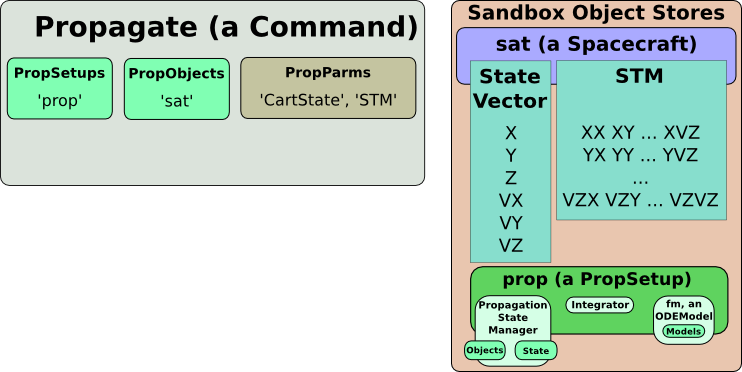
\includegraphics[371,186]{Images/PersistenceStart.png}
   \caption{Objects at the Start of the Propagate Command Initialization}
   \label{fig:PersistenceStart}
\end{figure}

Initialization for the Propagate command occurs after all of the resources defined in the script
have been cloned into the Sandbox and initialized.  The objects relevant to the command
initialization are shown in Figure~\ref{fig:PersistenceStart}.  The Sandbox object stores contain
the Spacecraft and PropSetup instances named as objects needed by the Propagate command.  Pointers
to these object stores are passed into the Propagate command immediately before the command is
initialized.  Then the initialization process is executed by a call from the Sandbox to the
Propagate command's Initialize() method.

\begin{figure}[htbp]
   \centering
   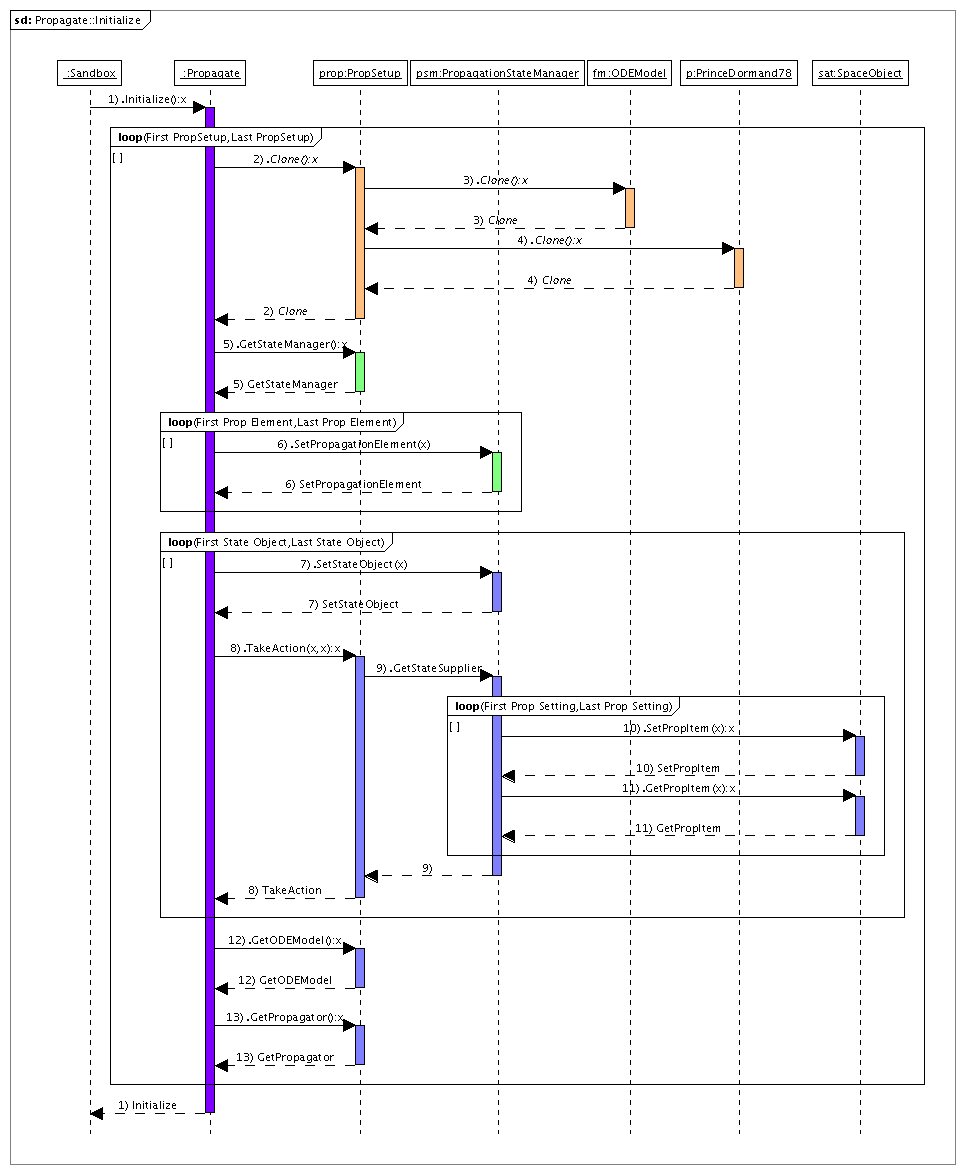
\includegraphics[460,560]{Images/PropagateInitialize.png}
   \caption{Steps Followed in the Propagate Command Initialization}
   \label{fig:PropagateInitialize}
\end{figure}

The steps followed in the Initialize() method are shown in Figure~\ref{fig:PropagateInitialize}.
The process illustrated starts when the Sandbox calls the Initialize() method on the Propagate
command. The command then loops through its list of PropSetups.  For each named PropSetup, the
command locates the associated object in one of ther Sandbox's object stores, and uses that copy to
make a local instance of the PropSetup for use by the command.  The local copy is made using the
PropSetup's Clone() method.  The Clone() method copies all of the internal PropSetup objects as
well, generating fresh instances of the Propagator and (for numerical integrators) ODEModel,
including all internal PhysicalModels.  Figure~\ref{fig:PersistenceCloned} shows the configuration
of the objects after this cloning has been completed.

\begin{figure}[htb]
   \centering
   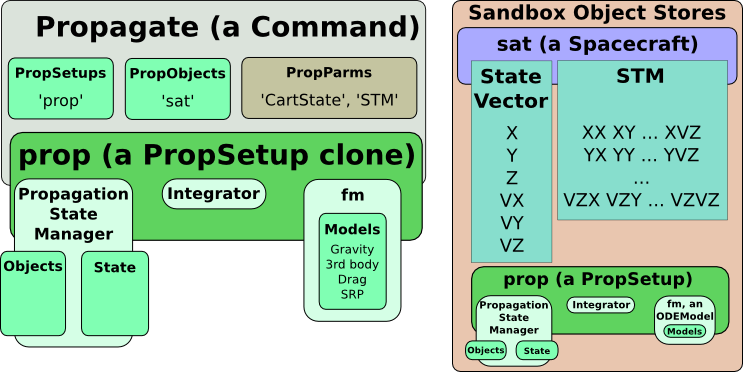
\includegraphics[372,186]{Images/PersistenceCloned.png}
   \caption{Objects after the Propagate Command Cloning}
   \label{fig:PersistenceCloned}
\end{figure}

Once the cloned copies of the PropSetup objects have been set in the PropSetup, the Propagate
command passes the list of propagation state elements needed to the PropSetup's propagation state
manager.  Then the command's initialization process iterates through the list of objects that need
to be propagated, setting their pointers on the PropSetup's propagation state manager.  For each of
these objects, the propagation state manager accesses and sets the pointers to the internal elements
that supply data for the propagation state vector.  This process, shown in the loop over state
objects on the figure, completes the elements of initializaton that can be performed prior to the
run of the mission.  The Propagate command then stores teh pointers to teh Propagator and ODEModel
in teh PropSetup for later use.  The resulting configuration is shown in
Figure~\ref{fig:PersistenceInitialized}; in this figure, pointers are prefaced by an ampersand (\&).

\begin{figure}[htb]
   \centering
   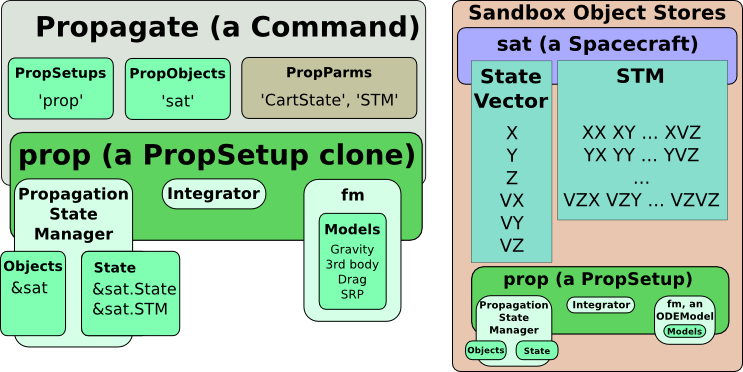
\includegraphics[372,186]{Images/PersistenceInitialized.png}
   \caption{Objects at Completion of the Propagate Command Initialization }
   \label{fig:PersistenceInitialized}
\end{figure}

\subsection{Preparing for Execution}

In GMAT, the components that are propagated can change based on actions taken as the mission is
run.  This feature allows for flexible configuration over the span of the mission, letting users
turn thrusters on and off, change ballistic properties of the objects, add new objects to , or
the set of objects being propagated, and toggle any other transient contributors to the
propagation model.  Because of this feature, the Propagate command delays the final setup for the
propagation state vector until immediately prior to performing propagation.  When a propagation
enabled command's Execute() method is called, the command finishes the setup process by calling a
member method, PrepareToPropagate(). The PrepareToPropagate() method performs the following tasks:

\begin{itemize}
\item Determines if any transient derivative model contributors have been activated
\item If so, adds these contributors to the ODE model
\item Adds any new elements to the set of objects being propagated
\item Constructs the propagation state vector
\item Sets the mapping between the propagation state vector and any ODE model being used
\item Fills the state data information, defining the initial state for the propagation
\end{itemize}


\begin{figure}[htb]
\centering
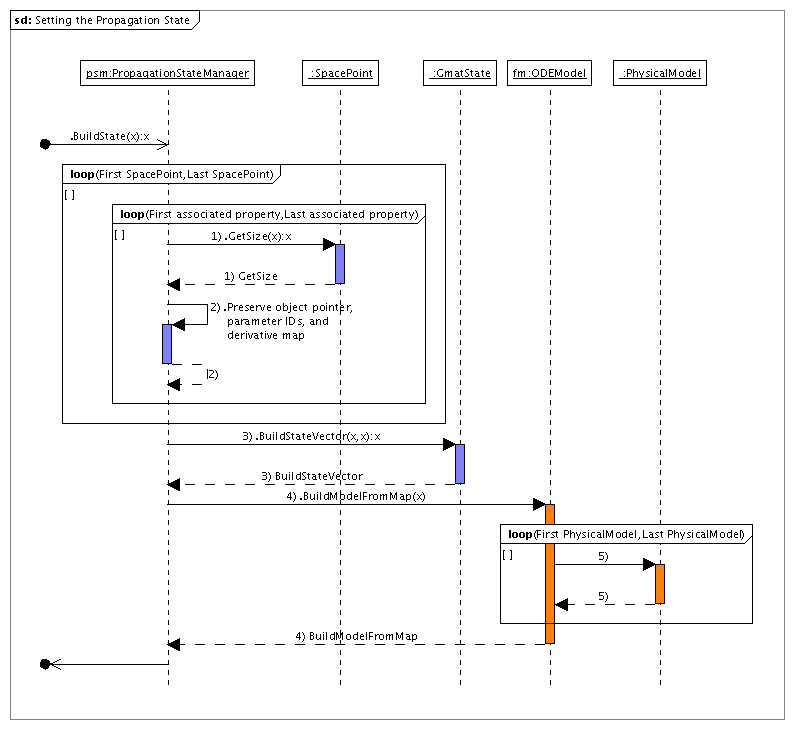
\includegraphics[380,335]{Images/SettingthePropagationState.png}
\caption{Details of the Steps Taken to Set Up the Propagation State and ODEModel}
\label{fig:P2PSetPropSate}
\end{figure}

\subsection{Execution}

\subsection{Finishing Up}

\section{The RunEstimator Command}

\section{The RunSimulator Command}

\begin{thebibliography}{99}

\bibitem{DesignPatterns} Gamma, Helm, Johnson, and Vlissides, \textbf{Design Patterns}, Addison
Wesley, 1995.
\bibitem{GMAT:2008} The GMAT Development Team, \textbf{General Mission Analysis Tool (GMAT)
Architectural Specification}, 2008.

\end{thebibliography}

\end{document}
